\documentclass[draft]{homework}

\usepackage{fixme}
\usepackage{graphicx}
\usepackage{xspace}

\newcommand{\dhcp}{DHCPv6\xspace}
\newcommand{\ip}{IPv6\xspace}
\newcommand{\opn}{OPNsense\xspace}


\title{Practical Network Defense - Lab 10}
\subtitle{\ip addressing of ACME co.’s network}
\author{Alessandro Serpi - 1647244}
\date{28 May 2019}


\begin{document}
    \maketitle
    \tableofcontents
    
    
    \pagebreak
    \section{Introduction}
    \fxnote{TODO}
    
    
    \section{Enabling \ip on the firewall}
    \fxnote{TODO}
    
    
    \section{Enabling \ip on the DMZ}
    The \dhcp server on DMZ interface must be configured with the prefix received on WAN: select \textit{Track Interface} in \textit{Interfaces} $\triangleright$ \textit{DMZ}, section \textit{\ip Configuration Type}.
    \begin{figure}[H]
        \centering
        
\includegraphics[width=\linewidth]{images/dmz-ipv6}
        \label{fig:dmz-ipv6}
    \end{figure}
    \vspace{-15pt}
    
    Leave the just-appeared options (in the bottom of the page) unchanged, only selecting WAN in \textit{\ip interface} if necessary.
    \begin{figure}[H]
        \centering
        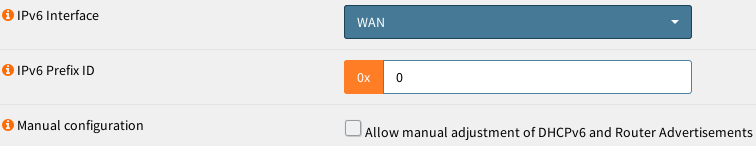
\includegraphics[width=\linewidth]{images/dmz-track}
        \label{fig:dmz-track}
    \end{figure}
    \vspace{-25pt}
    
    The relevant firewall rules are automatically added by \opn.
    
    
    \section{Test of the solution}
    \fxnote{TODO}
    
    
    \section{Final remarks}
    \fxnote{TODO}
\end{document}
